\section{Methods}
In this project, two different types of models were implemented and looked at. The baseline model pools the moves in each game together and predicts what the player was playing simply from the moves played in the game (without using information about the game position when the move was played or the order in which the moves were played). The main model of this study is a convolutional-LSTM model that captures the time element in the game, trying to learn patterns in the play to classify who is playing each game.

\subsection{Data Processing}
The raw data (see section \ref{data}) is in \href{https://en.wikipedia.org/wiki/Portable_Game_Notation}{Portable Game Notation} (.pgn) format, which is good for storing game metadata and the moves each player made during the game. When preprocessing the data, we stored the first 20 moves of each game, excluding shorter games, and stored it in a \verb$numpy$ array. For each game, we put together another array that included an ID of both players playing the game.
\medskip\par
The state of a chessboard can be represented in multiple ways. The way that was chosen for this project was to represent each move as a $24 \times 8 \times 8$ tensor of binary values. This is a similar representation of the moves as used in previous work (\citealp{main_article}), but we omit some of the excess information not related to the chess board.
Rhe first 12 channels represent what the board looked like before the move was made, and the later 12 channels represent the board after the move was made. Each board state is represented with 6 channels for the white pieces, one for the pawns, one for the rooks, one for the knights, one for the bishops, one for the queen, and one for the king. Similarly, the black pieces are represented with 6 channels. Figure \ref{fig:board_rep} shows an example of a board representation on the tensor form.

\setlength\arraycolsep{2pt}
\begin{figure}[ht!]
    \begin{subfigure}[c]{0.25\textwidth}
        \centering
        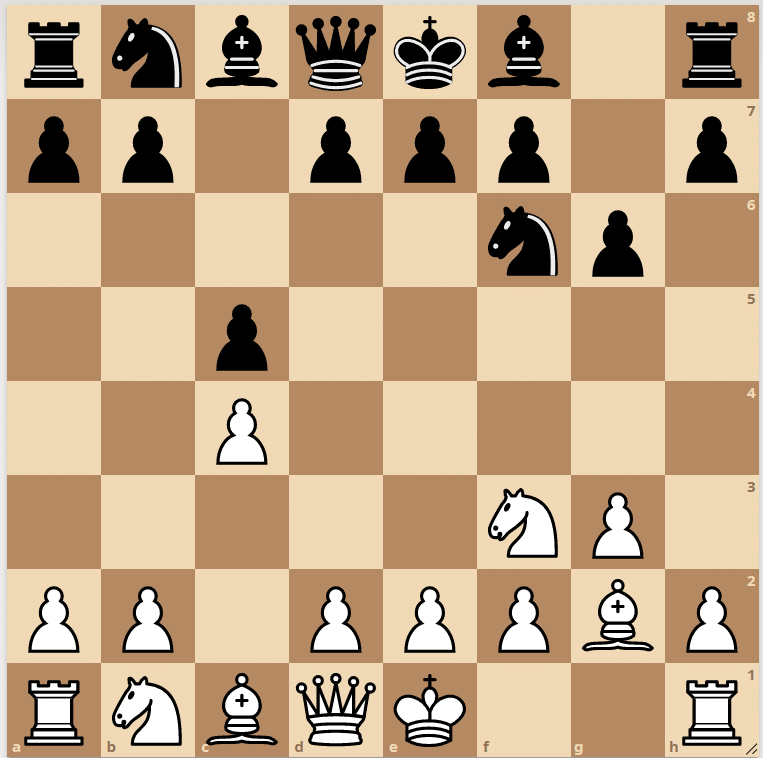
\includegraphics[width=3cm]{figures/board_state.png}
    \end{subfigure}%
    ~
    \begin{subfigure}[c]{0.74\textwidth}
        \centering
        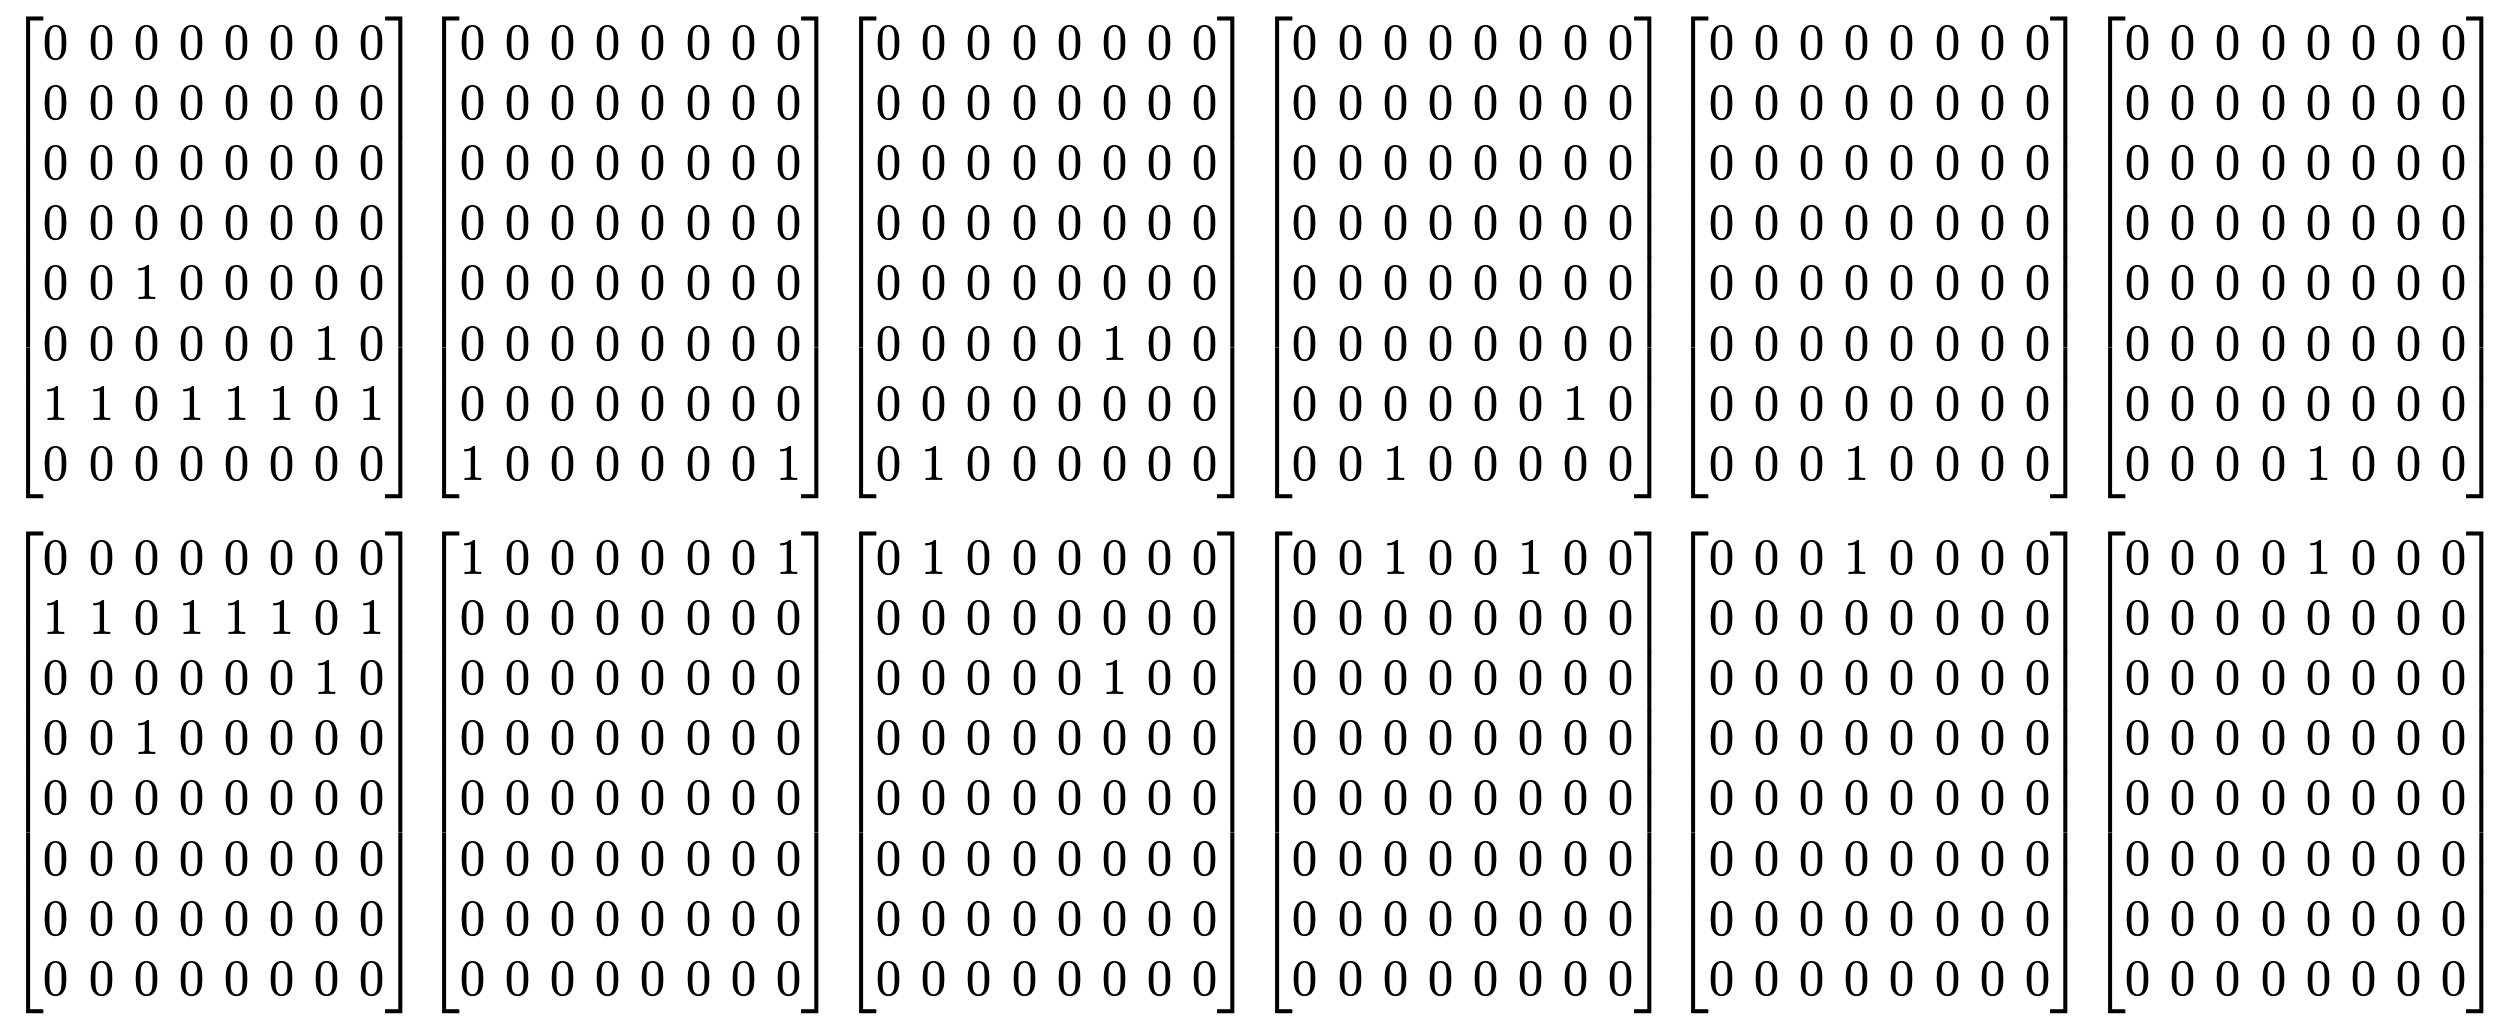
\includegraphics[width=4.5in]{figures/tensor-representation.png}
    % \begin{align*}
    %     &\scalemath{0.6}{
    %     \begin{bmatrix}
    %         0 & 0 & 0 & 0 & 0 & 0 & 0 & 0 \\
    %         0 & 0 & 0 & 0 & 0 & 0 & 0 & 0 \\
    %         0 & 0 & 0 & 0 & 0 & 0 & 0 & 0 \\
    %         0 & 0 & 0 & 0 & 0 & 0 & 0 & 0 \\
    %         0 & 0 & 1 & 0 & 0 & 0 & 0 & 0 \\
    %         0 & 0 & 0 & 0 & 0 & 0 & 1 & 0 \\
    %         1 & 1 & 0 & 1 & 1 & 1 & 0 & 1 \\
    %         0 & 0 & 0 & 0 & 0 & 0 & 0 & 0 \\
    %     \end{bmatrix}
    %     \begin{bmatrix}
    %         0 & 0 & 0 & 0 & 0 & 0 & 0 & 0 \\
    %         0 & 0 & 0 & 0 & 0 & 0 & 0 & 0 \\
    %         0 & 0 & 0 & 0 & 0 & 0 & 0 & 0 \\
    %         0 & 0 & 0 & 0 & 0 & 0 & 0 & 0 \\
    %         0 & 0 & 0 & 0 & 0 & 0 & 0 & 0 \\
    %         0 & 0 & 0 & 0 & 0 & 0 & 0 & 0 \\
    %         0 & 0 & 0 & 0 & 0 & 0 & 0 & 0 \\
    %          1 & 0 & 0 & 0 & 0 & 0 & 0 & 1 \\
    %     \end{bmatrix}
    %     \begin{bmatrix}
    %         0 & 0 & 0 & 0 & 0 & 0 & 0 & 0 \\
    %         0 & 0 & 0 & 0 & 0 & 0 & 0 & 0 \\
    %         0 & 0 & 0 & 0 & 0 & 0 & 0 & 0 \\
    %         0 & 0 & 0 & 0 & 0 & 0 & 0 & 0 \\
    %         0 & 0 & 0 & 0 & 0 & 0 & 0 & 0 \\
    %         0 & 0 & 0 & 0 & 0 & 1 & 0 & 0 \\
    %         0 & 0 & 0 & 0 & 0 & 0 & 0 & 0 \\
    %         0 & 1 & 0 & 0 & 0 & 0 & 0 & 0 \\
    %     \end{bmatrix}
    %     \begin{bmatrix}
    %         0 & 0 & 0 & 0 & 0 & 0 & 0 & 0 \\
    %         0 & 0 & 0 & 0 & 0 & 0 & 0 & 0 \\
    %         0 & 0 & 0 & 0 & 0 & 0 & 0 & 0 \\
    %         0 & 0 & 0 & 0 & 0 & 0 & 0 & 0 \\
    %         0 & 0 & 0 & 0 & 0 & 0 & 0 & 0 \\
    %         0 & 0 & 0 & 0 & 0 & 0 & 0 & 0 \\
    %         0 & 0 & 0 & 0 & 0 & 0 & 1 & 0 \\
    %         0 & 0 & 1 & 0 & 0 & 0 & 0 & 0 \\
    %     \end{bmatrix}
    %     \begin{bmatrix}
    %         0 & 0 & 0 & 0 & 0 & 0 & 0 & 0 \\
    %         0 & 0 & 0 & 0 & 0 & 0 & 0 & 0 \\
    %         0 & 0 & 0 & 0 & 0 & 0 & 0 & 0 \\
    %         0 & 0 & 0 & 0 & 0 & 0 & 0 & 0 \\
    %         0 & 0 & 0 & 0 & 0 & 0 & 0 & 0 \\
    %         0 & 0 & 0 & 0 & 0 & 0 & 0 & 0 \\
    %         0 & 0 & 0 & 0 & 0 & 0 & 0 & 0 \\
    %         0 & 0 & 0 & 1 & 0 & 0 & 0 & 0 \\
    %     \end{bmatrix}
    %     \begin{bmatrix}
    %         0 & 0 & 0 & 0 & 0 & 0 & 0 & 0 \\
    %         0 & 0 & 0 & 0 & 0 & 0 & 0 & 0 \\
    %         0 & 0 & 0 & 0 & 0 & 0 & 0 & 0 \\
    %         0 & 0 & 0 & 0 & 0 & 0 & 0 & 0 \\
    %         0 & 0 & 0 & 0 & 0 & 0 & 0 & 0 \\
    %         0 & 0 & 0 & 0 & 0 & 0 & 0 & 0 \\
    %         0 & 0 & 0 & 0 & 0 & 0 & 0 & 0 \\
    %         0 & 0 & 0 & 0 & 1 & 0 & 0 & 0 \\
    %     \end{bmatrix}} \\
    %     &\scalemath{0.6}{
    %     \begin{bmatrix}
    %         0 & 0 & 0 & 0 & 0 & 0 & 0 & 0 \\
    %         1 & 1 & 0 & 1 & 1 & 1 & 0 & 1 \\
    %         0 & 0 & 0 & 0 & 0 & 0 & 1 & 0 \\
    %         0 & 0 & 1 & 0 & 0 & 0 & 0 & 0 \\
    %         0 & 0 & 0 & 0 & 0 & 0 & 0 & 0 \\
    %         0 & 0 & 0 & 0 & 0 & 0 & 0 & 0 \\
    %         0 & 0 & 0 & 0 & 0 & 0 & 0 & 0 \\
    %         0 & 0 & 0 & 0 & 0 & 0 & 0 & 0 \\
    %     \end{bmatrix}
    %     \begin{bmatrix}
    %         1 & 0 & 0 & 0 & 0 & 0 & 0 & 1 \\
    %         0 & 0 & 0 & 0 & 0 & 0 & 0 & 0 \\
    %         0 & 0 & 0 & 0 & 0 & 0 & 0 & 0 \\
    %         0 & 0 & 0 & 0 & 0 & 0 & 0 & 0 \\
    %         0 & 0 & 0 & 0 & 0 & 0 & 0 & 0 \\
    %         0 & 0 & 0 & 0 & 0 & 0 & 0 & 0 \\
    %         0 & 0 & 0 & 0 & 0 & 0 & 0 & 0 \\
    %         0 & 0 & 0 & 0 & 0 & 0 & 0 & 0 \\
    %     \end{bmatrix}
    %     \begin{bmatrix}
    %         0 & 1 & 0 & 0 & 0 & 0 & 0 & 0 \\
    %         0 & 0 & 0 & 0 & 0 & 0 & 0 & 0 \\
    %         0 & 0 & 0 & 0 & 0 & 1 & 0 & 0 \\
    %         0 & 0 & 0 & 0 & 0 & 0 & 0 & 0 \\
    %         0 & 0 & 0 & 0 & 0 & 0 & 0 & 0 \\
    %         0 & 0 & 0 & 0 & 0 & 0 & 0 & 0 \\
    %         0 & 0 & 0 & 0 & 0 & 0 & 0 & 0 \\
    %         0 & 0 & 0 & 0 & 0 & 0 & 0 & 0 \\
    %     \end{bmatrix}
    %     \begin{bmatrix}
    %         0 & 0 & 1 & 0 & 0 & 1 & 0 & 0 \\
    %         0 & 0 & 0 & 0 & 0 & 0 & 0 & 0 \\
    %         0 & 0 & 0 & 0 & 0 & 0 & 0 & 0 \\
    %         0 & 0 & 0 & 0 & 0 & 0 & 0 & 0 \\
    %         0 & 0 & 0 & 0 & 0 & 0 & 0 & 0 \\
    %         0 & 0 & 0 & 0 & 0 & 0 & 0 & 0 \\
    %         0 & 0 & 0 & 0 & 0 & 0 & 0 & 0 \\
    %         0 & 0 & 0 & 0 & 0 & 0 & 0 & 0 \\
    %     \end{bmatrix}
    %     \begin{bmatrix}
    %         0 & 0 & 0 & 1 & 0 & 0 & 0 & 0 \\
    %         0 & 0 & 0 & 0 & 0 & 0 & 0 & 0 \\
    %         0 & 0 & 0 & 0 & 0 & 0 & 0 & 0 \\
    %         0 & 0 & 0 & 0 & 0 & 0 & 0 & 0 \\
    %         0 & 0 & 0 & 0 & 0 & 0 & 0 & 0 \\
    %         0 & 0 & 0 & 0 & 0 & 0 & 0 & 0 \\
    %         0 & 0 & 0 & 0 & 0 & 0 & 0 & 0 \\
    %         0 & 0 & 0 & 0 & 0 & 0 & 0 & 0 \\
    %     \end{bmatrix}
    %     \begin{bmatrix}
    %         0 & 0 & 0 & 0 & 1 & 0 & 0 & 0 \\
    %         0 & 0 & 0 & 0 & 0 & 0 & 0 & 0 \\
    %         0 & 0 & 0 & 0 & 0 & 0 & 0 & 0 \\
    %         0 & 0 & 0 & 0 & 0 & 0 & 0 & 0 \\
    %         0 & 0 & 0 & 0 & 0 & 0 & 0 & 0 \\
    %         0 & 0 & 0 & 0 & 0 & 0 & 0 & 0 \\
    %         0 & 0 & 0 & 0 & 0 & 0 & 0 & 0 \\
    %         0 & 0 & 0 & 0 & 0 & 0 & 0 & 0 \\
    %     \end{bmatrix}}
    % \end{align*}
    \end{subfigure}
    \caption{An example of a chess board representation. The channels of the tensor represent the board state of the image on top. The first 6 channels are for the white pieces, and channels 7-12 are for the black pieces. In the board representation that is put into the model, the state of the board before and after the move is used.}
    \label{fig:board_rep}
\end{figure}

\medskip\par
To create the tensor representation of the chess board we slightly modified code from Trevor Gaffa, in his \href{https://github.com/so-much-meta/lczero_tools/blob/master/src/lcztools/_leela_board.py}{lczero tools package}.

\medskip\par
In this way, each game is represented by a $n \times 24 \times 8 \times 8$ tensor, where $n$ represents the number of moves made in the game. For this project, $n = 20$ was chosen. We split each played game into games made with white pieces and games made with black pieces. 

\subsection{Convolutional LSTM Model}
\subsubsection{Model Structure}
The game-level data in each chess game is time-dependent, and the moves are played sequentially. Therefore, one thinks that the sequential nature of the data will help in predicting what player is playing. Our model is inspired by the work of \cite{main_article}, slightly simplified, using an LSTM model instead of a transformer to capture the sequential nature of the data. The embedding sizes and most hyperparameters are taken straight from their model. The model is composed of three main components. The first component is a CNN that each move is passed through, which changes the $24\times 8 \times 8$ tensor into a $64\times 1$ vector, followed by a fully connected layer to transform the result into a $320\times 1$ vector. The second component is an LSTM that takes in the representations created by the CNN model and outputs a $1024\times 1$ vector that is finally passed through to a fully connected layer that results in a $512\times 1$ representation of each game. The model learns these embeddings of chess games using a contrastive loss function called Generalized end-to-end loss (GE2E, see Section \ref{ge2e-section}). The idea of the G2E2 loss function comes from speaker recognition and rewards the model for keeping samples from the same player close together in the embedding space and samples from different players distant from each other.
%  To calculate the value of the loss function, $N$ players are sampled from the \emph{seen} players and $M$ games from each of those players are sampled in each batch to create an $N \times M \times 10 \times 24 \times 8 \times 8$ tensor. Here, $N$ and $M$ are hyperparameters but were chosen as $N = 10$ and $M = 10$.
\begin{figure}[ht!]
    \centering
    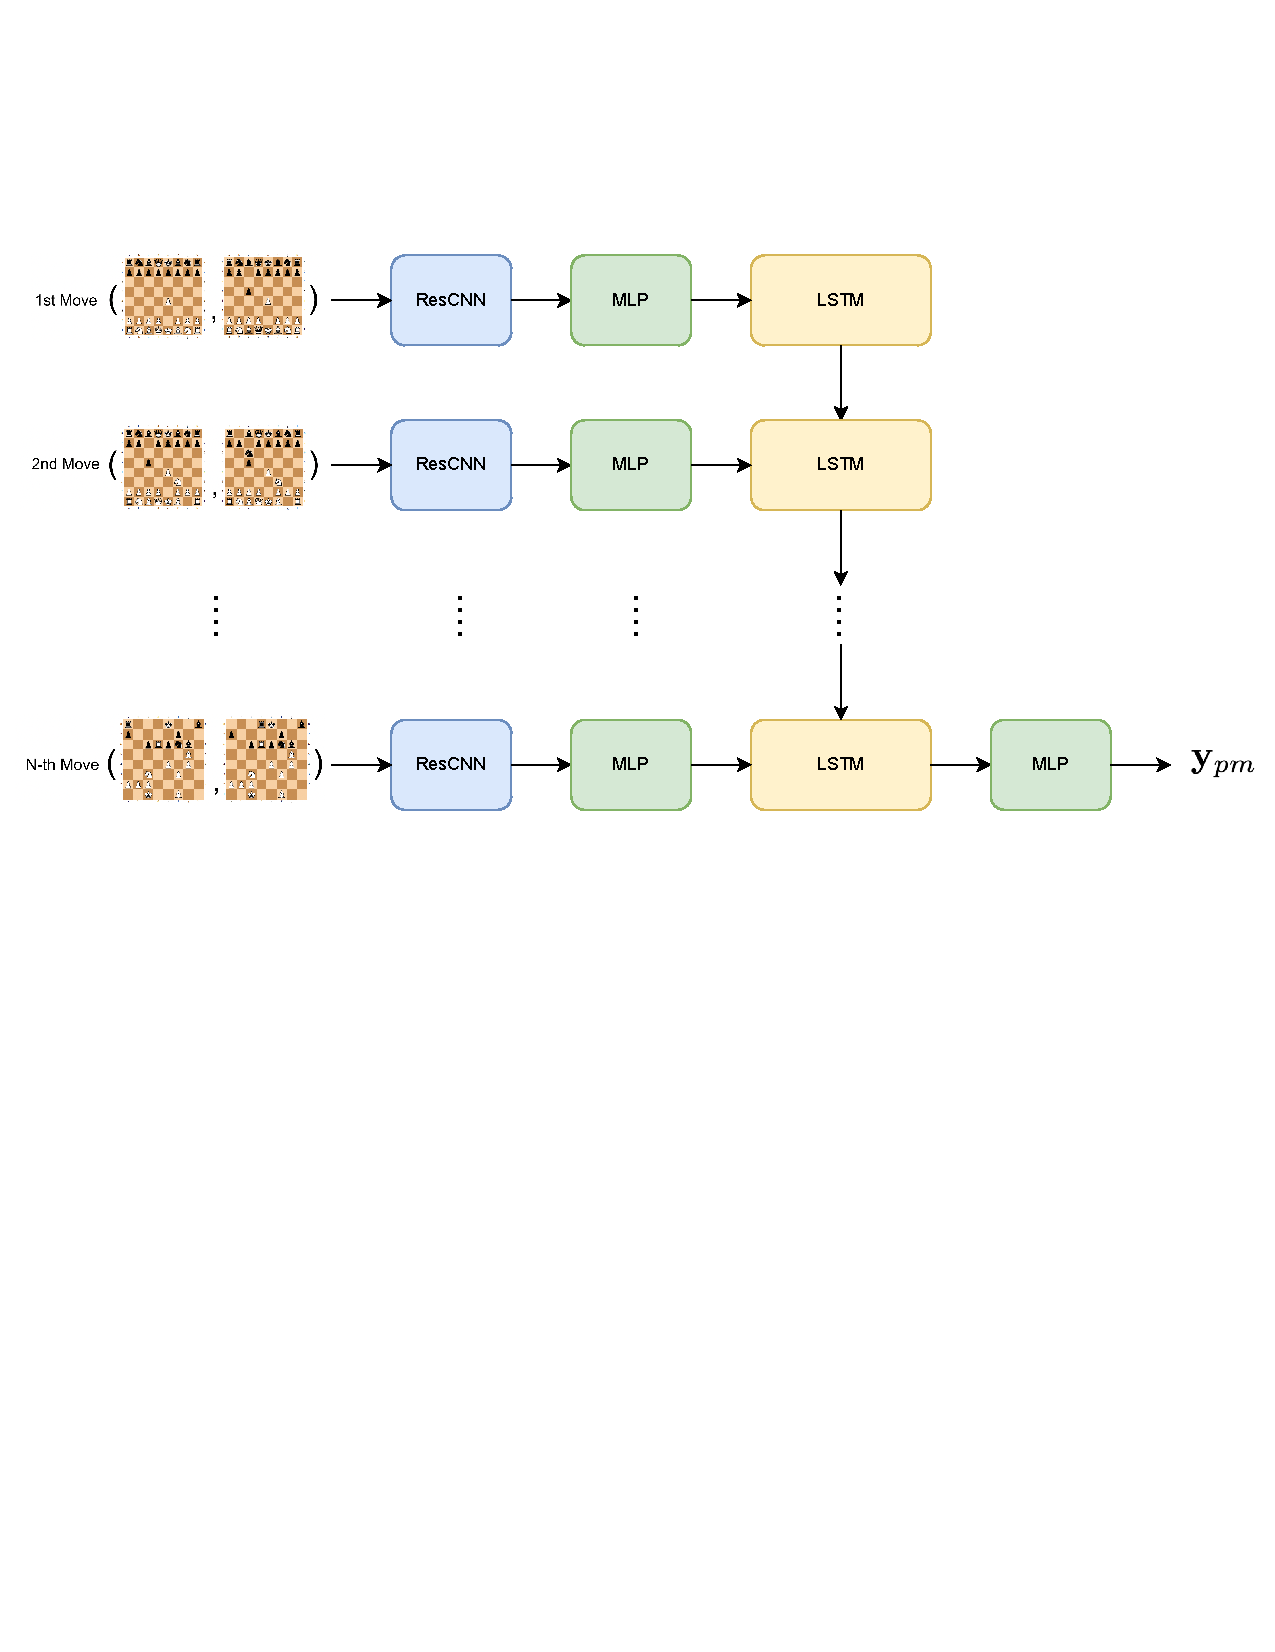
\includegraphics[width=0.9\textwidth]{figures/convLSTM.pdf}
    \caption{Visual representation of the convolutional LSTM model}
    \label{fig:convLSTM}
\end{figure}

\subsubsection{Residual Network Architecture}
We used a residual convolutional network to get a representation of a single move. The architecture was mainly inspired by the architecture used for this purpose in Maia, which is a chess engine designed to play like a human (\citealp{maia}). In our main model, we used one convolutional layer to convert from 24 channels to 64. Then there followed 6 residual blocks that conserve the dimension of the representation. 
The residual blocks consist of two convolutional layers with batch normalization after each one, and ReLU activation.
We used kernels of size $3\times 3$, a stride and zero padding of size one for all of the layers.
Finally, we used global average pooling to convert this to the shape of $64\times1\times1$. This was then fed through a fully connected layer whose output was the input to the LSTM. Figure \ref{fig:res_net} provides a visualization of this.

\begin{figure}[ht]
    \centering
    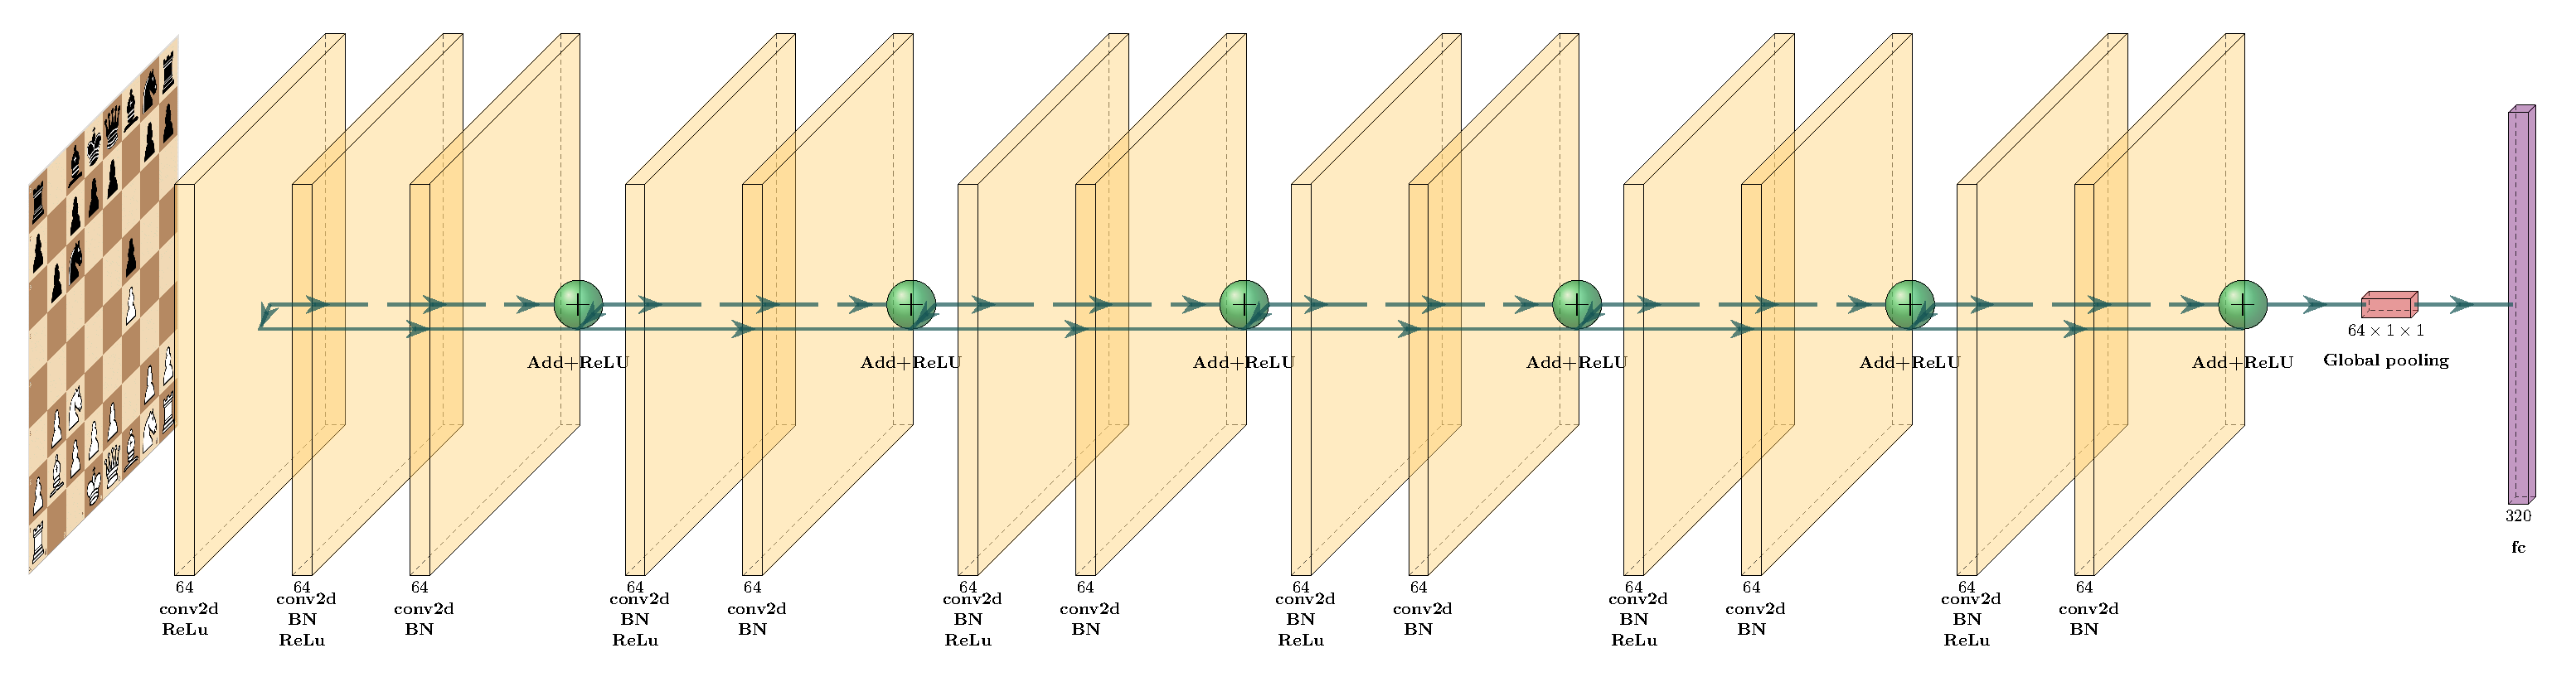
\includegraphics[width=6 in]{figures/Tilraun.pdf}
    \caption{Visualization of the residual network used for processing the moves}
    \label{fig:res_net}
\end{figure}

\subsubsection{Generalized End-to-End Loss} \label{ge2e-section}
Since the model is an embedding model, a classic softmax/MSE optimization does not suffice. A contrastive loss function must be implemented (\citealp{ge2e}). In each training batch, $M$ games are sampled from each of $N$ random players from the pool of players. Following the notation from \cite{main_article}, we denote the embedding of game $m$ of player $p$ with $\mathbf{y}_{pm}$. When the loss function is calculated, the centroids $\mathbf{c}_p = \frac{1}{M}\sum_{m=1}^M\mathbf{y}_{pm}$ are calculated. Further, the modified centroids 
\[\mathbf{c}_{p}^{(-i)} = \frac{1}{M-1}\sum_{\substack{m = 1 \\ m \neq i}}^M\mathbf{y}_{pm}\]
are calculated. These modified centroids are used to compare the distance from a single game to the other games that the player played. If we included the game we are looking at in that centroid, that game would pull the centroid closer to itself. Figure \ref{fig:ge2e-visualization} visualizes the concepts of $\mathbf{c}_p$, $\mathbf{c}_p^{(-m)}$ and $\mathbf{y}_{pm}$.
\begin{figure}[ht]
    \centering
    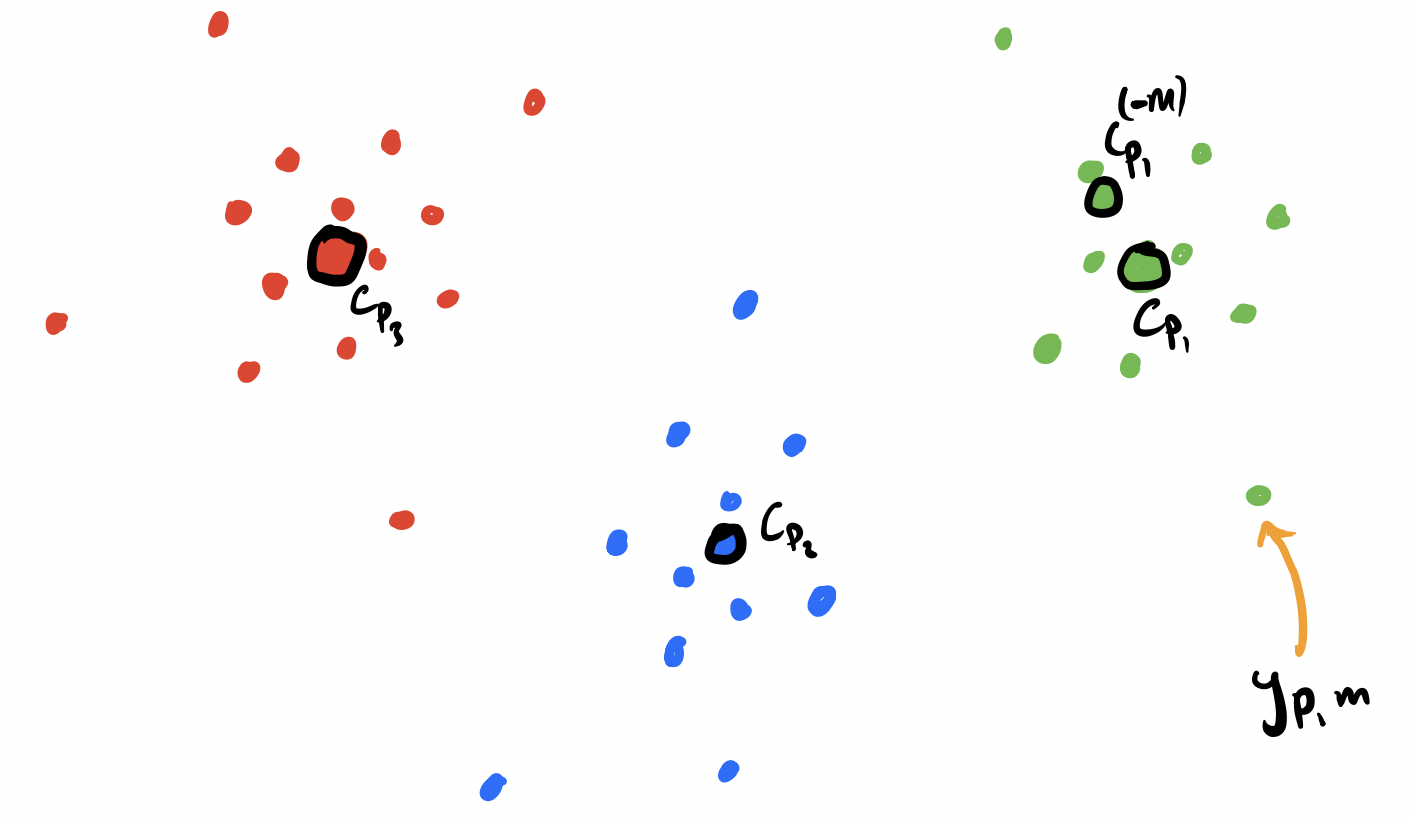
\includegraphics[width=0.7\textwidth]{figures/ge2e-visualization.png}
    \caption{Visual representation of the embeddings and their centroids. The points with black border represent centroids, the upper green centroid is the modified centroid w.r.t. the sample the arrow points at.}
    \label{fig:ge2e-visualization}
\end{figure}
\medskip\par 
We define a similarity matrix $\mathbf{S}_{pm, q}$, where $p$ represents the player that played the game and $q$ means that we are comparing this game to the games played by player $q$, as
\begin{align*}
    \mathbf{S}_{pm,q} = \begin{cases}
        w\cos(\mathbf{y}_{pm}, \mathbf{c}_p^{(-m)}) + b, &\text{if } p = q \\
        w\cos(\mathbf{y}_{pm}, \mathbf{c}_q) + b, & \text{otherwise},
    \end{cases}
\end{align*}
where $w$ and $b$ are learned parameters and $\cos$ is the cosine similarity function. This similarity matrix measures the similarity between a game and the centroids of the players in the batch. As we want to maximize the distance to other players and minimize the distance to the player that played the game, the loss of the sample is defined as
\[L(\mathbf{y}_{pm}) = -S_{pm, p} + \log\sum_{q=1}^N\exp(\mathbf{S}_{pm,q}).\]
Finally, the loss of the batch is defined as
\[L = \sum_{p=1}^N\sum_{m=1}^ML(\mathbf{y}_{pm}).\]
The generalized end-to-end code was taken straight from Harry Volek's \href{https://github.com/HarryVolek/PyTorch_Speaker_Verification}{PyTorch Speaker Verification} project on GitHub.

\subsection{$k$-shot Learning Routine}
\label{k-shot}
To achieve the goal of making the model generalize well to unseen players, we use prototypical learning (\citealp{Prototypical_learning}).
The model learns a mapping from the moves played in a game to a high-dimensional embedding space. The desirable mapping is one that clusters the samples from each player together.
At test time, we calculate the embeddings of all of the samples in the reference sets (see section \ref{train-test}). We create a prototype for each player by taking the centroid of their vectors. To predict who is playing in a sample from the query set, the model calculates the embedding of that sample and outputs the player whose prototype is closest to the embedding.

\subsection{Baseline Model}
To validate the results of our convolutional LSTM model, we created a simple baseline model inspired by \cite{main_article}. To do that, we used an ad hoc approach in creating the embedding vectors. The model calculates the embedding for each sample by $n$-hot encoding the first $n$ moves, i.e., the moves that the player played in the first $n$ moves are encoded with 1, and all other possible moves are encoded with 0. Note that we do not take into account the position in which the move was played. For example, if white played the knight from b8 to c6, we do not take into account whether this move was played in the first move or the $n$-th move.
Here $n$ is a hyperparameter. The prototypes for each player and predictions are then calculated as described in section \ref{k-shot}.
This method takes advantage of the fact that in chess, players often use the same memorized opening moves.

\subsection{Data}\label{data}
The data that was used in this project comes from chess games played on \href{https://lichess.org/}{Lichess}. It was possible to download every game played on Lichess, but the files for that data were around 30 Gb for each month, which would take too long to parse. After some searching, we found the \href{https://database.nikonoel.fr/}{Lichess Elite Database}, a database that has been gathered since 2013 of games where players with a Lichess rating of 2400 or higher played against players with a Lichess rating of 2200 or higher, excluding bullet games. For this project, at most 100,000 games per month in the year 2019 were used, totaling around 800,000 games in the dataset. After creating the train/test split (see Section \ref{train-test}), the training data comprised of just under 400,000 games.

% For the convLSTM model we want it to have knowledge of the board position when given a move. To do so, we encode the board position after each move and store it in Forsyth–Edwards Notation (.fen) format which is a single string that encodes the board at each time. The .fen encoding is then converted to a tensor. We treat each game as two sequences, one for the white pieces and one for the black ones. Each point in the sequence is two tensors, one corresponding to the board position before the move was made on one for the position after the move. From the metadata in the .pgn file we can retrieve the name of the players and their Elo points which will be used as the targets in the model. 

\subsubsection{Train/Test Split} \label{train-test}
To measure the quality of the model, we use two measures. The first goal was to be able to predict who is playing a given chess game out of the players the model was trained on. For the model to be generalizable, we also want to measure the accuracy of the model on previously unseen players, using only a few of their games as points of reference.
\medskip\par
First off, the players were split into \emph{seen} and \emph{unseen} players. The \emph{seen} players are the 400 players with the most amount of games in the dataset, ranging from 950 to 9000 games played in the year 2019. The \emph{unseen} players were the players that were not in the top 400 in games played but had played over 100 games in the year 2019. 
\medskip\par 
To create the final splits for the dataset, 100 games from each \emph{seen} player were reserved for test time, and the model was trained on the rest of their data. Out of these 100 games, 50 games were reserved for a reference set, a set to calculate the centroids of the players, and a query set, a real test set to measure the accuracy of the model. For the unseen players, the same split was created for 100 games that they played at random.

\subsubsection{Training Time Sampling}
Since the training dataset consists of almost 400,000 games, we could not create the tensor representation for every game in the dataset beforehand (that would result in having to store $400000\cdot2\cdot20\times24\times8\times8 = 2.5 \cdot 10^9   $ binary values in memory). Therefore, the tensor representations must be created during training time. 
\medskip\par
Each batch is sampled at training time as well. The input into the generalized end-to-end loss function (see section \ref{ge2e-section}) must be on the format $N \times M \times D$, where $N$ represents the number of players looked at in the batch, $M$ the number of games per player in each batch, and $D$ the embedding size of each game. This means that we have to pass in a tensor of size $N \times M \times  n \times 24 \times 8 \times 8$ into the model, where $n$ represents the number of moves looked at per game. To create this tensor, $N$ players at random were chosen to compare with each other, and $M$ games from each of these players were sampled for comparison. For each of these games, the tensor representation was created and fed into the model.

